\documentclass[8pt]{beamer}
\usetheme{Pittsburgh}
%\usecolortheme{lily}
\usepackage{amsmath,amssymb,amsfonts,amsthm}
\usepackage{graphicx}
\usepackage[skins,theorems]{tcolorbox}
\usepackage{epsfig}
\usepackage{verbatim}
\usepackage{textpos}
\usepackage{subfigure}
\usepackage{beamertexpower}
\usepackage{multirow}
\usepackage{hhline}
\usepackage{array}
\usepackage{booktabs}
\usepackage{tikz}
\usepackage{bm}
\usepackage{etoolbox}
\usepackage{caption}
\usepackage{natbib}
\usepackage{color,colortbl}
\usepackage[ruled]{algorithm2e}
\usepackage{bm}
\usepackage{interval}
\usetikzlibrary{arrows,shapes}
\newcommand{\highlight}[1]{\colorbox{yellow!80!gray}{$\displaystyle #1$}}
\newcommand{\highlightG}[1]{\colorbox{green!50!white}{$\displaystyle #1$}}
\newcommand{\highlightR}[1]{\colorbox{red!50!white}{$\displaystyle #1$}}

%\captionsetup[figure]{labelformat=empty}


\definecolor{CASgray}{RGB}{196,196,188}
\definecolor{CASblue}{RGB}{50,70,123}
\definecolor{CASred}{RGB}{198,78,78}
\definecolor{CASgreen}{RGB}{114,164,104}

\setbeamertemplate{enumerate item}{%
  \usebeamercolor[bg]{item projected}%
  \raisebox{1.5pt}{\colorbox{black!60!white}{\color{fg}\footnotesize\insertenumlabel}}%
}


\usepackage{pgfplots}
\pgfplotsset{compat=newest}
\pgfplotsset{plot coordinates/math parser=false}
\newlength\figureheight
\newlength\figurewidth
\definecolor{Gray}{gray}{0.9}

\setbeamercolor{title}{fg=black!80!white,bg=black!5!white} 
\setbeamertemplate{footline}{\hfill\insertframenumber/\inserttotalframenumber}
%\useoutertheme{smoothbars}
\usefonttheme{professionalfonts}
%\usefonttheme{serif}
%\usepackage[]{palatino}
%\usepackage{eulervm}
%\usefonttheme{structuresmallcapsserif}
%\usefonttheme{serif}
%\setbeamercolor{palette tertiary}{use=structure,bg=black!95!blue}
%\usepackage{mathpazo} % add possibly `sc` and `osf` options
%\usepackage{eulervm}
\newcolumntype{g}{>{\columncolor{Gray}}c}

\title[Efficient Visual-Inertial Navigation using IMU Pre-integration]{\huge Efficient Visual-Inertial Navigation using IMU Pre-integration}

\author[Liyang Liu]{\large {Liyang} Liu\vskip0.3cm}%, \textbf{Kasra Khosoussi}}
\institute[CAS]{\large Centre for Autonomous Systems\\[0.2cm]University of
  Technology Sydney\vskip0.3cm
%  
\includegraphics[width=3cm]{UTS-logo}
%  \hspace{2cm}
%  \includegraphics[width=1.5cm]{cas-logo}
%  \vskip0.5cm
}

%\date{Robotics: Science and Systems 2015}
% Ignore these lines
%%%%%%%%%%%%%%%%%%%%%%%%%%%%%%%%%%%%%%%%%%%%%%%%%%%%%%%%%%%%%%%%%%%%%%%%%%%%%%%%%%%%%%%%%%%%%%%%%%%%%%%%
%%%%%%%%%%%%%%%%%%%%%%%%%%%%%%%%%%%%%%%%%%%%%%%%%%%%%%%%%%%%%%%%%%%%%%%%%%%%%%%%%%%%%%%%%%%%%%%%%%%%%%%%
%%%%%%%%%%%%%%%%%%%%%%%%%%%%%%%%%%%%%%%%%%%%%%%%%%%%%%%%%%%%%%%%%%%%%%%%%%%%%%%%%%%%%%%%%%%%%%%%%%%%%%%%
%%%%%%%%%%%%%%%%%%%%%%%%%%%%%%%%%%%%%%%%%%%%%%%%%%%%%%%%%%%%%%%%%%%%%%%%%%%%%%%%%%%%%%%%%%%%%%%%%%%%%%%%
%%%%%%%%%%%%%%%%%%%%%%%%%%%%%%%%%%%%%%%%%%%%%%%%%%%%%%%%%%%%%%%%%%%%%%%%%%%%%%%%%%%%%%%%%%%%%%%%%%%%%%%%
\setbeamertemplate{navigation symbols}{} 
%\setbeamercolor{section in head/foot}{fg=CASgray,bg=CASblue}
%\setbeamercolor{subsection in head/foot}{fg=CASblue,bg=CASgray}
%%\setbeamercolor{frametitle}{bg=CASblue!70!white,fg=CASgray!30!white}
\setbeamercolor{frametitle}{bg=white,fg=black!70!white}%CASgray!30!white}
%\setbeamercolor{title}{bg=CASblue!80!white}
\setbeamertemplate{itemize items}[triangle]
%\setbeamertemplate{enumerate items}[default]
%\setbeamercolor{itemize item}{fg=CASblue!80!white}
\setbeamercolor{enumerate item}{fg=red}
%\setbeamercolor{section number projected}{bg=CASblue!80!white,fg=white}
%\setbeamercolor{section in toc}{fg=CASblue!80!white}
\setbeamercolor{block title}{bg=white!90!blue}
\setbeamercolor{block body}{bg=CASgray!10!white}
%\setbeamercolor{block title alerted}{bg=CASred,fg=white}
%\setbeamercolor{block body alerted}{bg=CASred!10!white}
%\setbeamercolor{block title example}{bg=CASgreen!80!white,fg=white}
\setbeamertemplate{headline}{}
%\AtBeginEnvironment{alertblock}{\setbeamercolor{itemize item}{fg=CASred}}
%\AtBeginEnvironment{exampleblock}{\setbeamercolor{itemize item}{fg=CASgreen}}

\setbeamertemplate{title page}[default][colsep=-1bp,rounded=true]
\setbeamertemplate{blocks}[rounded][shadow=false]

%\AtBeginSection[]
%{
%  \begin{frame}
%    \frametitle{Table of Contents}
%    \tableofcontents[currentsection]
%  \end{frame}
%}

%\usefonttheme{serif} 
%\usepackage{mathpazo} % math & rm
%\linespread{1.1}        % Palatino needs more leading (space between lines)
%\normalfont
%\usepackage[T1]{fontenc}

%\logo{%
%%    \includegraphics[width=0.65cm,height=0.65cm,keepaspectratio]{cas-logo}
%    
\includegraphics[width=0.6cm]{figures/UTS-small}
%}


%\addtobeamertemplate{frametitle}{\vskip-0.8ex}{}
%\setbeamertemplate{headline}{%
%\leavevmode%
%  \hbox{%
%    \begin{beamercolorbox}[wd=\paperwidth,ht=1.5ex,dp=1.125ex]{subsection in
%	  head/foot}%
%    %\insertsectionnavigationhorizontal{\paperwidth}{}{\hskip0pt plus1filll}
%    \end{beamercolorbox}%
%  }
%}
%\defbeamertemplate*{footline}{infolines theme}
%{
%  \leavevmode%
%  \hbox{%
%%  \begin{beamercolorbox}[wd=.5\paperwidth,ht=2.25ex,dp=1ex,center]{subsection in head/foot}%
%%    \usebeamerfont{author in head/foot}\insertshortauthor
%%  \end{beamercolorbox}%
%%  \begin{beamercolorbox}[wd=.40\paperwidth,ht=2.25ex,dp=1ex,center]{author in head/foot}%
%%    \usebeamerfont{title in head/foot}\insertshorttitle
%%  \end{beamercolorbox}%
%  \begin{beamercolorbox}[wd=1\paperwidth,ht=2.25ex,dp=1ex,right]{bg=white,fg=CASblue}%
%    \insertframenumber{}\hspace*{2ex} 
%  \end{beamercolorbox}
%  }%
%  \vskip0pt%
%}


%\setbeamertemplate{footline}[page number]{}



\titlegraphic{
  \vspace{0.1cm}
  
\includegraphics[width=3cm]{figures/UTS-logo}
  \hspace*{2.7cm}

\includegraphics[width=2.4cm]{figures/UTS_CAS.pdf}
}


%\setbeamertemplate{headline}
%{
%  \leavevmode%
%  \hbox{%
%  \begin{beamercolorbox}[wd=\paperwidth,ht=8.25ex,dp=3.5ex]{secsubsec}%
%    \raggedright
%    \hspace*{2em}%
%    {\sffamily\Large\color{CASgreen}\thesection.~\insertsection\hfill\insertsubsection}%
%    \hspace*{2em}%
%  \end{beamercolorbox}%
%  }%
%}
\setbeamertemplate{frametitle}
{\vskip-3pt
  \leavevmode
  \hbox{%
  \begin{beamercolorbox}[wd=\paperwidth,ht=3ex,dp=1ex]{frametitle}%
    \raggedright\hspace*{1em}\insertframetitle
  \end{beamercolorbox}
  }%
}

\addtobeamertemplate{frametitle}{}{%
\begin{textblock*}{100mm}(.94\textwidth,-0.82cm)

\includegraphics[height=0.6cm]{figures/UTS_CAS.pdf}
\end{textblock*}}


\makeatletter
  \def\vhrulefill#1{\leavevmode\leaders\hrule\@height#1\hfill \kern\z@}
\makeatother

\setbeamerfont{frametitle}{size=\huge,series=\bfseries}
%\setbeamertemplate{frametitle}{\color{CASblue!85!CASgray}\bfseries\insertframetitle\par\vskip-2pt}%\vhrulefill{1pt}}

\setbeamerfont{title}{series=\bfseries}
\setbeamerfont{block title}{series=\bfseries}
%%%%%%%%%%%%%%%%%%%%%%%%%%%%%%%%%%%%%%%%%%%%%%%%%%%%%%%%%%%%%%%%%%%%%%%%%%%%%%%%%%%%%%%%%%%%%%%%%%%%%%%%
%%%%%%%%%%%%%%%%%%%%%%%%%%%%%%%%%%%%%%%%%%%%%%%%%%%%%%%%%%%%%%%%%%%%%%%%%%%%%%%%%%%%%%%%%%%%%%%%%%%%%%%%
%%%%%%%%%%%%%%%%%%%%%%%%%%%%%%%%%%%%%%%%%%%%%%%%%%%%%%%%%%%%%%%%%%%%%%%%%%%%%%%%%%%%%%%%%%%%%%%%%%%%%%%%
%%%%%%%%%%%%%%%%%%%%%%%%%%%%%%%%%%%%%%%%%%%%%%%%%%%%%%%%%%%%%%%%%%%%%%%%%%%%%%%%%%%%%%%%%%%%%%%%%%%%%%%%
%%%%%%%%%%%%%%%%%%%%%%%%%%%%%%%%%%%%%%%%%%%%%%%%%%%%%%%%%%%%%%%%%%%%%%%%%%%%%%%%%%%%%%%%%%%%%%%%%%%%%%%%
%%%%%%%%%%%%%%%%%%%%%%%%%%%%%%%%%%%%%%%%%%%%%%%%%%%%%%%%%%%%%%%%%%%%%%%%%%%%%%%%%%%%%%%%%%%%%%%%%%%%%%%%
\begin{document}



\begin{frame}[plain]
  \titlepage
\end{frame}


\begin{frame}{Visual Inertial SLAM}
  \tableofcontents
\end{frame}

\section{Introduction}
\section{Preintegration as parameterization on Z}
\section{Covariance and Jacobain calculation of Preintegration}
\section{IMU Bias treatment}
\section{Experimental results}

% page - introduction
\begin{frame}{Introduction}
	
	\begin{figure}[!ht]
		\begin{center}\begin{tabular}{cc}
				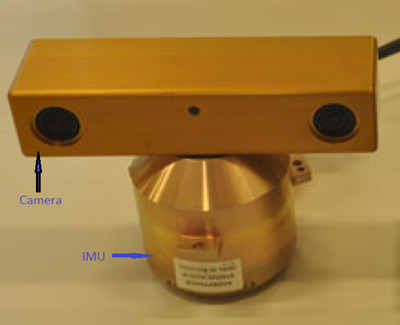
\includegraphics[height=3.3cm]{figures/bumblebee_imu.png}&
				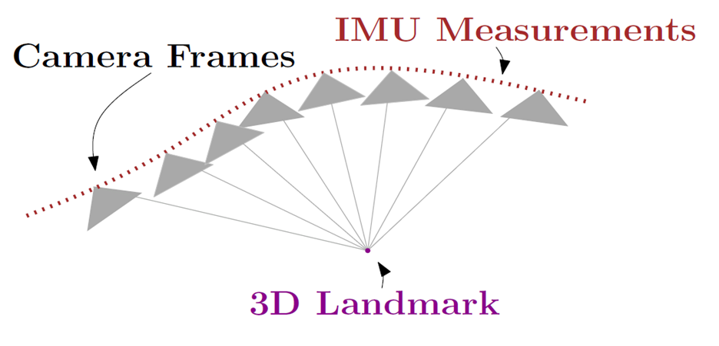
\includegraphics[height=3.3cm]{Figures/IMU-sample_Image-frames_3D_illustration.png}\\
				(a) & (b) \\
		\end{tabular}\end{center}
		\caption{\emph{a}) Sensors: Camera+IMU \cite{Tod2012}, \emph{b}) Sensor information \cite{Manifold2015}} 
		\label{fig:VIN sensor information}
	\end{figure} 
	
  \begin{figure}[ht]
  	%    \centering
  	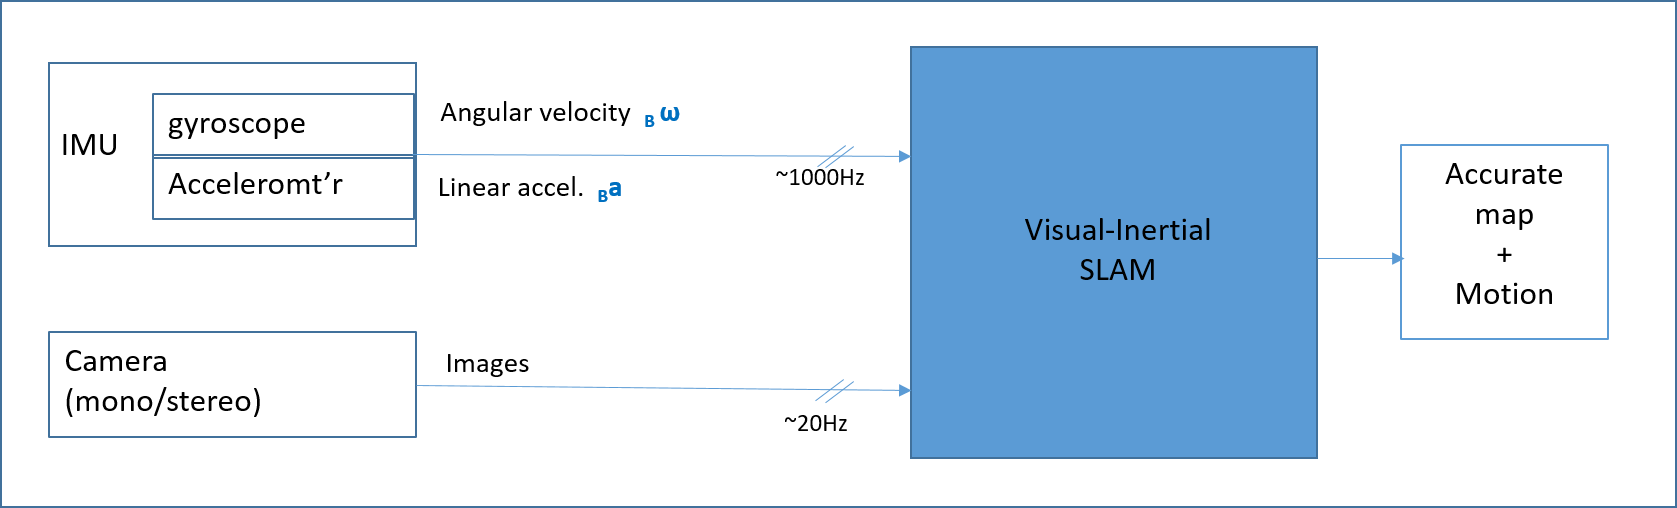
\includegraphics[width=9cm]{figures/vin_data_flow.png}
  	\caption{VIN data flow}
  \end{figure}
	
\end{frame}

% page - Explanation of VIN problem
\begin{frame}{The Vin problem}
\begin{table}[ht!]
	\begin{center}\begin{tabular}{  p{6cm}  p{6cm} }
			\multirow{2}{*}{
				\raisebox{-\totalheight}{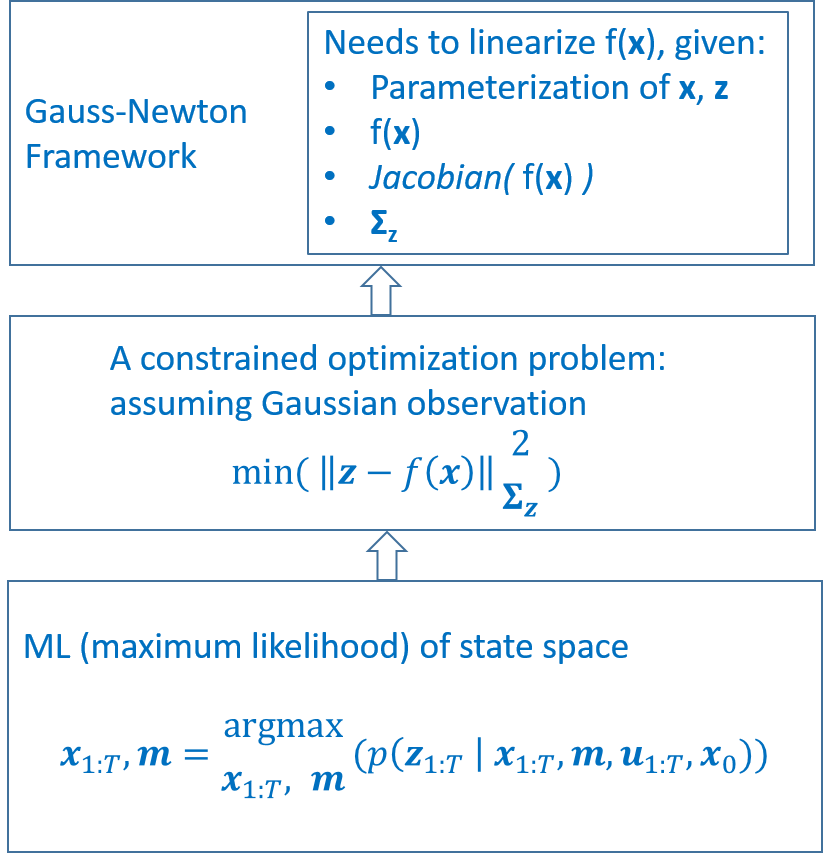
\includegraphics[height=4.5cm]{figures/Graph_Slam_theory.png}}}			
			&
			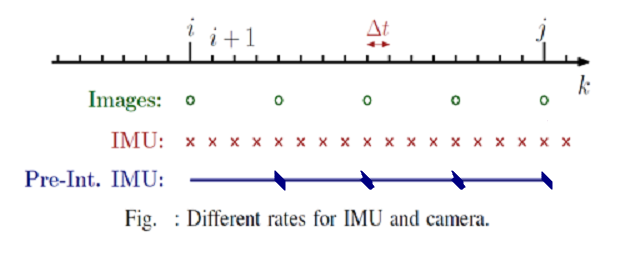
\includegraphics[height=2cm]{figures/IMU-Image_different-sample-rate_time-series-illustration.png} 
			\\
			{} 
			& 
			\begin{itemize}
				\item Naïve parameterization:
				\begin{itemize}
					\item $\bm{x}$: pose, orientation, velocity $\{R_t,  \mathrm{{}_{w}}\bm{p}_{t},  \mathrm{{}_{w}}\bm{v}_{t}  \}, t \in \left[0, T_{total} \right]$ for all IMU smpls
					
					\item $\bm{z}$: all IMU data points $\{  \mathrm{{}_{B}}\bm{\omega}_{t},  \mathrm{{}_{B}}\bm{a}_{t} \}$ and all feature observations $\{\bm{z}_{il}\}, i \in I_{total}, l \in C_{i}$\\
					{\tiny $I_{total}$ : all images, $C_l$ : correspondences in frm $i$, $\mathrm{{}_{B}}$ : body frame}
					
					\item $\Sigma_{\bm{z}}$: $\eta^g$ - angular rate noise, $\eta^a$ - linear acc noise, $\eta^i$ - image uv noise
					
				\end{itemize}
				\item Infeasible: 
				\begin{itemize}
					\item Too much observation data					
					\item Re-compute integration at each new linearization (e.g. rotation $R_t$ ).
					
				\end{itemize}
			\end{itemize} 
			
		\end{tabular}\end{center}
	\end{table}			
\end{frame}

% page - Preintegration as a solution

\begin{frame}{Example}
  \begin{itemize}
    \item example 1
    \item example 2
  \end{itemize}

  \begin{block}{Title}
    normal block -- colors can be changed easily
  \end{block}

  \begin{equation}
    \sum \log (x_i)
    \label{}
  \end{equation}

	
  \begin{figure}[hl]
%    \centering
    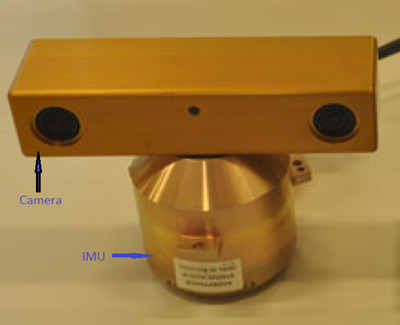
\includegraphics[width=3cm]{figures/bumblebee_imu.png}
    \caption{Sensors: Camera + IMU}
  \end{figure}
  
  
\end{frame}





\end{document}
